\documentclass{article}

\usepackage[
backend=biber,
style=numeric,
sorting=ynt
]{biblatex}
\addbibresource{refs.bib}

\usepackage{parskip}
\usepackage{colortbl}
\usepackage{soul}
\usepackage{ifthen}
\usepackage[makeroom]{cancel}
\usepackage{amsthm}
\usepackage{amsmath}
\usepackage{amssymb}
\usepackage{mathtools}
\usepackage{needspace}
\usepackage{etoolbox}
\usepackage{listofitems}
\usepackage{xstring}
\usepackage{graphicx} % Required for inserting images
\usepackage{tikz}
\usetikzlibrary{arrows.meta}
\usetikzlibrary{patterns}
\usetikzlibrary{external}
\usetikzlibrary{decorations.pathreplacing}
\usetikzlibrary{decorations.markings}

\usepackage{arydshln}
\setlength{\dashlinedash}{2pt}  % Finer dashes
\setlength{\dashlinegap}{2pt}     % Smaller gaps

\newtheorem{theorem}{Theorem}
\newtheorem{definition}{Definition}
\newtheorem{lemma}{Lemma}

\preto{\theorem}{\needspace{3cm}}
\preto{\lemma}{\needspace{3cm}}
\preto{\section}{\needspace{7cm}}
\preto{\subsection}{\needspace{3cm}}
\preto{\definition}{\needspace{3cm}}

\title{\vspace{-2cm}\includegraphics[scale=0.6]{birkhoff_heart.pdf}\\\vspace{0.5cm} Heart of the Four Color Theorem}
\author{Timothy van der Valk}
\date{January 2025, Tohoku University}

\definecolor{g0}{RGB}{150, 255, 150}
\newcommand{\bir}{\text{Bir}\Diamond}
\newcommand{\ber}{\text{Ber}\Diamond}
\newcommand*\circled[1]{\tikz[baseline=(char.base)]{\node[shape=circle,draw,inner sep=1pt] (char) {#1};}}
\newcommand{\chain}[3]{#1 \stackrel{#3}{\frown} #2 }
\newcommand{\confg}{\mathcal{C}}
\newcommand{\core}{\mathcal{K}}
\newcommand{\I}{\text{I}}
\newcommand{\II}{\text{II}}
\newcommand{\compat}{\implies}
\newcommand{\ncompat}[1]{\stackrel{#1}{\compat}}
\newcommand{\digitToNum}[1]{\the\numexpr#1\relax}
\newcommand{\scheme}[2]{
    \readlist*\mylist{#2}
     \tikz[baseline]{ 
        \foreach \x [count=\i] in {#1} {
            \coordinate (\i) at (0.3*\i, 0.225); \node[text height=0mm] at (0.3*\i,0) {$\x$};
        } 
        \foreachitem \z \in \mylist {
            \StrChar{\z}{1}[\left]
            \StrChar{\z}{2}[\right]
            \StrChar{\z}{3}[\color]
            \StrChar{\z}{4}[\cross]
            \path (\left) edge[bend left=45] node[above, yshift=-2]{\small 
            \ifthenelse{\equal{\cross}{-}}{$\cancel{\color}$}{$\color$}
            } (\right);
        }
    }
} 

\begin{document}

\maketitle

The four color theorem is a famous result from graph theory that has resisted proof for well over a 100 years. An application of this theorem states that any world map can be colored with four colors in such a way, that two neighboring regions receive different colors. When tasked with coloring a map, the solution lies in the idea of breaking the map into smaller pieces that are easy to color. This idea is called \textit{reducibility}. This paper gives an intuitive and step by step explanation of the three forms of reducibility used in the proof of the four color theorem. 

We first explain how maps with regions arranged in a \textit{ring} can broken up into smaller maps. This idea is first introduced by Birkhoff in 1913 \cite{birkhoff}. We have simplified his proofs for the reducing of rings of 4 and 5 regions using clear language and new notation. From rings, we move on to breaking up maps that contain special arrangments of regions within them called \textit{configurations}. This brings us to D-reducibility and C-reducibility of configurations. Each form of reducibility motivates the next, and with that, the whole notion of reducibility is motivated from a single, simple idea.
\vspace{0.1cm}\\
{ \tiny Title image - The Birkhoff diamond shaped like a heart (original). }

\pagebreak

\pagebreak
\section*{Summary}
\label{sec:summary}

The four color theorem states that every map can be colored with four colors in such a way, that two neighboring regions receive different colors. Such a coloring is desired for a world map, because it becomes easy to tell two neighboring regions apart. It has been observed by many map makers that four colors suffice. The problem was first formulated by Francis Guthrie in 1852 while coloring the map of England. He brought the problem to his brother Frederick Guthrie, who in turn brought the problem to his mathematics lecturer Augustus De Morgan. 

At the heart of the famous proof of the four color theorem by Appel and Haken in 1976 \cite{appel} is shown that the problem of coloring any map can be reduced to the coloring of a map with less regions. By repeating this result on the smaller map, the coloring problem eventually turns trivial. The two key concepts used in showing this are 1. \textit{Reducibility} and 2. \textit{Unavoidability}. 

Reducibility develops the theory about breaking maps up into smaller pieces that are easier to color. There are three forms of reducibility used in the four color theorem. Each builds upon the previous.

\begin{enumerate}
\item \textit{Ring-reducibility} breaks up maps that contain \textit{rings} of regions surrounding other regions. It is shown that the interior and exterior regions of certain rings can always be colored in such a way that the colors match on the ring. This allows us to color the interior and exterior seperately, hence breaking the map into two pieces. 

\item \textit{D-reducibility} builds upon Ring-reducibility. Given a ring in a map with a certain arrangement of regions on the interior called a \textit{configuration}, it is shown that any coloring outside of the ring can be extended to match a coloring for the inside. 

\item \textit{C-reducibility} extends upon D-reducibility by first replacing the configuration with a smaller \textit{reducer}. The colorings of the reducer can then be extended to match the original configuration.
\end{enumerate}

\textit{Unavoidability} builds upon the concept of configurations. Here it is shown that it is \textit{unavoidable} that a map contains a configuration or ring that is reducible. Therefore every map can be broken down into pieces that are trivial to color. This part uses the \textit{discharge method} to prove a certain finite set of configurations is unavoidable in a map. A computer is then used to check that each of these configurations (well over 600, 1400 or even 2800 of them) is in fact, reducible.

The first proof of the four color theorem had a set of 1478 configurations to check. An improvement was made by Neil Robertson et al. \cite{thomas} in 1996 who reduced the set to only 633 configurations that are either C or D-reducible. Lastly, an improvement was made by John P. Steinberger in 2009 who used only D-reducibility at the cost of having to check 2822 configurations. A proof that does not utilize a computer is still unavailable.

\tableofcontents

\pagebreak
\section{Introduction}
\label{sec:intro}

\subsection{Graph coloring}

The four color theorem was initially formulated from a problem in coloring world maps. A map consists of regions that can border other regions on a flat surface. When we talk about a \textit{coloring} of a map, we mean a way to color its regions such that any two neighbors are colored differently.

The actual shape of the regions in our map is not of importance here. The key information that is needed from a map, is the connectivity between regions. Such information can be represented in a \textit{graph} where vertices (circles) correspond to regions. An edge between two vertices then indicates that the two corresponding regions are neighbors.

\begin{figure}[!h]
    \centering
    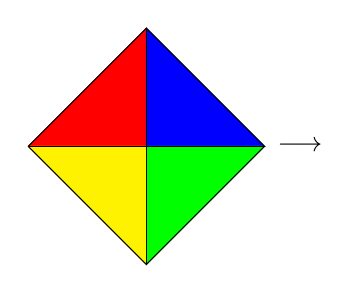
\begin{tikzpicture}[scale=1.5]
        \coordinate (v1) at (-1, 0);
        \coordinate (v2) at (0, 1);
        \coordinate (v3) at (1, 0);
        \coordinate (v4) at (0, -1);
        \coordinate (c) at (0, 0);

        \draw [fill, red] (v1) -- (v2) -- (c) -- (v1);
        \draw [fill, blue] (v2) -- (v3) -- (c) -- (v2);
        \draw [fill, green] (v3) -- (v4) -- (c) -- (v3);
        \draw [fill, yellow] (v4) -- (v1) -- (c) -- (v4);
        \draw (v1) -- (v2) -- (v3) -- (v4) -- (v1);
        \draw (c) -- (v1);
        \draw (c) -- (v2);
        \draw (c) -- (v3);
        \draw (c) -- (v4);
        \node at (1.3, 0) { $\longrightarrow$ };
    \end{tikzpicture} 
    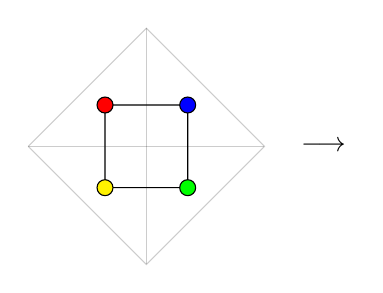
\begin{tikzpicture}[scale=1.5]
        \coordinate (v1) at (-1, 0);
        \coordinate (v2) at (0, 1);
        \coordinate (v3) at (1, 0);
        \coordinate (v4) at (0, -1);
        \coordinate (c) at (0, 0);

        \node[circle, fill, scale=0.01cm, red, draw=black] (m1) at (-0.35, 0.35) { $v_1$ };
        \node[circle, fill, scale=0.01cm, blue, draw=black] (m2) at (0.35, 0.35) { $v_2$ };
        \node[circle, fill, scale=0.01cm, green, draw=black] (m3) at (0.35, -0.35) { $v_3$ };
        \node[circle, fill, scale=0.01cm, yellow, draw=black] (m4) at (-0.35, -0.35) { $v_4$ };

        \draw (m1) -- (m2) -- (m3) -- (m4) -- (m1);
        \draw[opacity=0.2] (v1) -- (v2) -- (v3) -- (v4) -- (v1);
        \draw[opacity=0.2] (c) -- (v1);
        \draw[opacity=0.2] (c) -- (v2);
        \draw[opacity=0.2] (c) -- (v3);
        \draw[opacity=0.2] (c) -- (v4);
        \node at (1.5, 0) { $\longrightarrow$ };
    \end{tikzpicture}  
    \begin{tikzpicture}[scale=1.5, mid arrow/.style={
        postaction={ decorate, decoration={ markings, mark=at position 0.6 with { \arrow[black]{>>} } } } }]
        \coordinate (v1) at (-1, 0);
        \coordinate (v2) at (0, 1);
        \coordinate (v3) at (1, 0);
        \coordinate (v4) at (0, -1);
        \coordinate (c) at (0, 0);

        \node[circle, fill, scale=0.015cm, label=above left:$a$] (m1) at (-0.35, 0.35) { };
        \node[circle, fill, scale=0.015cm, label=above right:$b$] (m2) at (0.35, 0.35) { };
        \node[circle, fill, scale=0.015cm, label=below right:$c$] (m3) at (0.35, -0.35) { };
        \node[circle, fill, scale=0.015cm, label=below left:$d$] (m4) at (-0.35, -0.35) { };

        \draw[mid arrow] (m1) -- (m2);
        \draw (m2) -- (m3) -- (m4) -- (m1);
        \draw[opacity=0.0] (v1) -- (v2) -- (v3) -- (v4) -- (v1);
    \end{tikzpicture}      
    \caption{The translation of a map coloring to a graph coloring. In the last step we replace colors by the letters $a$,$b$,$c$ and $d$ for convenience. We obtain the coloring called $abcd$. The edge $\gg$ indicates the order of the coloring in case of ring-shaped graphs. }
    \label{fig:colortut}
\end{figure}

From now on, we will leave the notion of maps and regions behind us and work solely with graphs. The four color theorem can then be formulated as follows.

\begin{theorem}
    Every planar graph can be colored in at most four colors.
\end{theorem}

With \textit{planar graph} we mean a drawing of a graph as in the left-most graph of Figure \ref{fig:colortut}. Edges are not allowed to cross each other. The proof of this theorem required over a 100 years to complete, despite its simple statement. What would you do to prove such a statement? You would first try very hard for one day. After that, you move on to a weaker variant of the statement. This brings us to the five color theorem.
\subsection{The five color theorem}
A weaker variant of the four color theorem is the five color theorem. It simply states that every planar graph can be colored in at most five colors instead of four.

\begin{theorem}
    Every planar graph can be colored in at most five colors.
\end{theorem}

\begin{proof}
Given a planar graph $G$. Because $G$ is planar, a known result in graph theory is that $G$ has a vertex with at most five edges. That is, there is a $v$ such that $deg(v) \leq 5$. If we can always free up a color for $v$ regardless of the colors of its neighbors, then we may simply ignore $v$ for now and color the smaller graph $G-v$ first. By repeating the same argument on $G-v$ and so on, we will eventually be left with just a single vertex. From there we can build up the 5-coloring of our graph.

Therefore, let us show that we can always free up a color for $v$. We consider two cases for $\deg(v) \leq 5$.

\begin{itemize}
    \item $\deg(v) \leq 4$. In this case, our vertex has at most four neighbors. These four neighbors have at most four different colors. This means that one color is free to be used for $v$.
    \item $\deg(v) = 5$. In this case, we have exactly five neighbors. Should our neighbors require only four colors, we can simply use our fifth color here. However, it might occur that all five neighbors use all five colors. Now we must try to free up a color in these neighbors.
\end{itemize}

Indeed, to treat the case $\deg(v)=5$ we should make a sketch of the situation first.

\begin{figure}[!h]
    \centering
    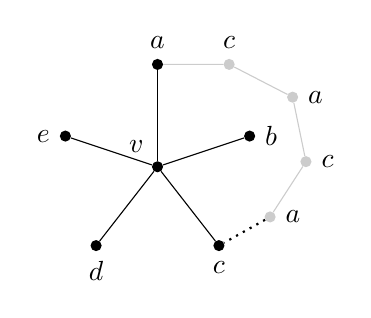
\begin{tikzpicture}[scale=1.3]
        \node[circle, fill, scale=0.015cm, label=above left:$v$] (c) at (0, 0) {};
        \node[circle, fill, scale=0.015cm, label=above:$a$] (l1) at (0, 1) { };
        \node[circle, fill, scale=0.015cm, label=right:$b$] (l2) at (0.9, 0.30) { };
        \node[circle, fill, scale=0.015cm, label=below:$c$] (l3) at (0.6, -0.77) {};
        \node[circle, fill, scale=0.015cm, label=below:$d$] (l4) at (-0.6, -0.77) {};
        \node[circle, fill, scale=0.015cm, label=left:$e$] (l5) at (-0.9, 0.30) {};
        \node[circle, fill, scale=0.015cm, label=above:$c$, opacity=0.2] (c1) at (0.7, 1) {};
        \node[circle, fill, scale=0.015cm, label=right:$a$, opacity=0.2] (c2) at (1.32, 0.68) {};
        \node[circle, fill, scale=0.015cm, label=right:$c$, opacity=0.2] (c3) at (1.45, 0.05) {};
        \node[circle, fill, scale=0.015cm, label=right:$a$, opacity=0.2] (c4) at (1.1, -0.49) {};

        \draw (c) -- (l1);
        \draw (c) -- (l2);
        \draw (c) -- (l3);
        \draw (c) -- (l4);
        \draw (c) -- (l5);

        \draw[opacity=0.2] (l1) -- (c1) -- (c2) -- (c3) -- (c4);
        \draw[dotted, thick] (c4) -- (l3);
        
    \end{tikzpicture}
    \label{fig:5colthm}
    \caption{The vertex $v$ when having five differently colored neighbors. In gray, an example $ac$-chain starting from the neighbor $a$. }
\end{figure}

Now we must ask ourselves, do these neighbors really need to use all five colors?
We may flip all the vertices colored $a$ or $c$ that are connected to the top neighbor $a$ to change its color to $c$. This way we freed up the color $a$. We say that we flipped the $ac$\textit{-chain} of neighbor $a$. Such a chain can be seen in Figure \ref{fig:5colthm}.

However, if the neighbor $c$ is part of this $ac$-chain (represented by a dotted line), then it will get flipped to $a$. So in this case we have not freed up the color $a$. We did however, isolate the vertex $b$ with the $ac$-chain. It is now impossible for a $bd$-chain from $b$ to $d$ to exist. Therefore we can flip the $bd$-chain of  $b$ to change its color into $d$ without affecting the neighbor $d$. This frees up the color $b$.

Therefore, all cases show that a color can be freed up for $v$. By our earlier argument the graph is 5-colorable.
\end{proof}

\subsection{Fundaments of the four color theorem}

The proof of the four color theorem follows the same structure as the five color theorem. We show that every planar graph contains a subgraph that allows us to reduce the coloring problem to a smaller graph. This notion of a \textit{subgraph} of a graph requires some extra attention, since there are multiple ways to be a subgraph.

Given a subgraph $\confg$ of a planar graph $G$. There are roughly two ways that $\confg$ can be a subgraph of $G$. See Figure \ref{fig:containtut}.

\begin{figure}[!ht]
    \centering
    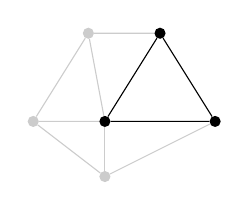
\begin{tikzpicture}[scale=0.7]
        \node[circle, fill, scale=0.015cm] (l1) at (-1, 0) { };
        \node[circle, fill, scale=0.015cm] (l2) at (1, 0) { };
        \node[circle, fill, scale=0.015cm] (l3) at (0, 1.6) {};

        \node[circle, fill, scale=0.015cm, opacity=0.2] (e1) at (-1.3, 1.6) { };
        \node[circle, fill, scale=0.015cm, opacity=0.2] (e2) at (-2.3, 0) { };
        \node[circle, fill, scale=0.015cm, opacity=0.2] (e3) at (-1, -1) { };

        \draw (l1) -- (l2) -- (l3) -- (l1);
        \draw[opacity=0.2] (e1) -- (l1) -- (e2);
        \draw[opacity=0.2] (e3) -- (l1);
        \draw[opacity=0.2] (l3) -- (e1) -- (e2) -- (e3) -- (l2);
    \end{tikzpicture}
    \hspace{1cm}
    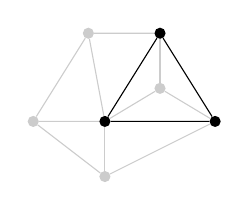
\begin{tikzpicture}[scale=0.7]
        \node[circle, fill, scale=0.015cm] (l1) at (-1, 0) { };
        \node[circle, fill, scale=0.015cm] (l2) at (1, 0) { };
        \node[circle, fill, scale=0.015cm] (l3) at (0, 1.6) {};

        \node[circle, fill, scale=0.015cm, opacity=0.2] (e1) at (-1.3, 1.6) { };
        \node[circle, fill, scale=0.015cm, opacity=0.2] (e2) at (-2.3, 0) { };
        \node[circle, fill, scale=0.015cm, opacity=0.2] (e3) at (-1, -1) { };

        \node[circle, fill, scale=0.015cm, opacity=0.2] (w1) at (0, 0.6) { };

        \draw (l1) -- (l2) -- (l3) -- (l1);
        \draw[opacity=0.2] (w1) -- (l1);
        \draw[opacity=0.2] (w1) -- (l2);
        \draw[opacity=0.2] (w1) -- (l3);
        \draw[opacity=0.2] (e1) -- (l1) -- (e2);
        \draw[opacity=0.2] (e3) -- (l1);
        \draw[opacity=0.2] (l3) -- (e1) -- (e2) -- (e3) -- (l2);
    \end{tikzpicture}
    \caption{Strong containment (left) is an exact copy of a graph $\confg$ in $G$. Weak containment (right) might have additional vertices on the interior of $\confg$.}
    \label{fig:containtut}
\end{figure}

\begin{definition}
    A planar graph $\confg$ is \emph{strongly-contained} in a graph $G$ if no vertices of $G$ are in the interior of $\confg$. Otherwise, $\confg$ is \emph{weakly-contained}.
\end{definition}

Naturally, the form of containment that we will be working with is strong containment. This gives a clear seperation between the interior and exterior of a contained graph $\confg$. With that, we will define what it means for such a graph $\confg$ to be reducible.

\begin{definition}
    A planar graph $\confg$ is \emph{reducible} in a graph $G$ if $\confg$ being strongly-contained in $G$ implies that the 4-coloring of $G$ can be reduced to the 4-coloring of $G'$ with less vertices. $\confg$ is called a \emph{configuration}.
\end{definition}

Now we are ready to phrase the result that lies at the heart of the four and five color theorem.

\begin{theorem}
    \label{funda1}
    Every planar graph $G$ strongly-contains a configuration $\confg$ that is either $k$-reducible, D-reducible or C-reducible in $G$.
\end{theorem}

From this theorem, a 4-coloring of a planar graph $G_0$ can be found as follows. A worked example of this algorithm can be found in Section \ref{sec:algorithm}.

\begin{enumerate}
    \item Find a reducible configuration $C_n$ in $G_n$.
    \item Reduce the graph $G_n$ to the smaller graph $G_{n+1}$.
    \item If $G_{n+1}$ is the empty graph, color all the intermediate graphs starting from $G_n$ all the way until $G_0$, else, repeat Step 1 on $G_{n+1}$.
\end{enumerate}

This process is indeed the same as the repetition argument we gave in the five color theorem. We will now introduce the first concept of reducibility inspired by the five color theorem. 
\section{$k$-Reducibility}
\label{sec:ringreduce}

\subsection{Rings}
\label{subsec:rings}

We have seen in the proof of the five color theorem that a vertex surrounded by five or less neighbors can always be colored using one of five colors, even if all of its neighbors initially use all five colors. If we have only four colors available, we will find that it is no longer guaranteed that we can free a color. This is what Alfred Kempe tried to do when he gave the first false proof of the four color theorem.

If we look at the key idea, we see that if one half of a graph is isolated from another half by a group of boundary vertices, we can color this isolated part regardless of the colors on the boundary. Naturally, the fundamental shape that seperates a graph in two halves is a \textit{ring} (or a line if it is not cyclic).

\begin{definition}
    A \emph{ring} of $n$ vertices $R_n$ in a planar graph $G$ is an induced cycle of $G$.
\end{definition}

An example of what is a ring and what is not can be seen in Figure \ref{fig:ring}.

\begin{figure}[!ht]
    \centering
    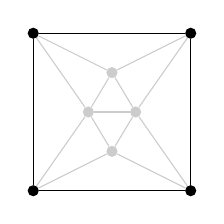
\begin{tikzpicture}
        \node[circle, fill, scale=0.015cm] (l1) at (-1, -1) { };
            \node[circle, fill, scale=0.015cm] (l2) at (-1, 1) { };
            \node[circle, fill, scale=0.015cm] (l3) at (1, 1) {};
            \node[circle, fill, scale=0.015cm] (l4) at (1, -1) {};
            \node[circle, fill, scale=0.015cm, opacity=0.2] (m1) at (0, 0.5) {};
            \node[circle, fill, scale=0.015cm, opacity=0.2] (m2) at (-0.3, 0) {};
            \node[circle, fill, scale=0.015cm, opacity=0.2] (m3) at (0.3, 0) {};
            \node[circle, fill, scale=0.015cm, opacity=0.2] (m4) at (0, -0.5) {};

            \draw (l1) -- (l2) -- (l3) -- (l4) -- (l1);
            \draw[opacity=0.2] (m1) -- (m2) -- (m4) -- (m3) -- (m1);
            \draw[opacity=0.2] (m2) -- (m3);
            \draw[opacity=0.2] (m1) -- (l2);
            \draw[opacity=0.2] (m1) -- (l3);
            \draw[opacity=0.2] (m2) -- (l1);
            \draw[opacity=0.2] (m2) -- (l2);
            \draw[opacity=0.2] (m3) -- (l3);
            \draw[opacity=0.2] (m3) -- (l4);
            \draw[opacity=0.2] (m4) -- (l1);
            \draw[opacity=0.2] (m4) -- (l4);
    \end{tikzpicture}
    \hspace{1cm}
    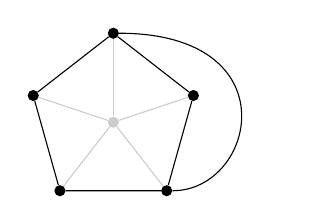
\begin{tikzpicture}[scale=1.13]
        \node[circle, fill, scale=0.015cm, opacity=0.2] (c) at (0, 0) {};


        \node[circle, fill, scale=0.015cm] (l1) at (0, 1) { };
        \node[circle, fill, scale=0.015cm] (l2) at (0.9, 0.30) { };
        \node[circle, fill, scale=0.015cm] (l3) at (0.6, -0.77) {};
        \node[circle, fill, scale=0.015cm] (l4) at (-0.6, -0.77) {};
        \node[circle, fill, scale=0.015cm] (l5) at (-0.9, 0.30) {};

        \draw[opacity=0.2] (c) -- (l1);
        \draw[opacity=0.2] (c) -- (l2);
        \draw[opacity=0.2] (c) -- (l3);
        \draw[opacity=0.2] (c) -- (l4);
        \draw[opacity=0.2] (c) -- (l5);
        \draw (l1) -- (l2) -- (l3) -- (l4) -- (l5) -- (l1);
        \draw (l1) .. controls +(2,0) and +(1,0) .. (l3);
    \end{tikzpicture}
    \caption{In bold, an example of the ring $R_4$ surrounding a graph on four vertices (left) and an example of an invalid ring $R_5$. No extra edges are allowed between ring vertices, since otherwise the ring is not an induced cycle of $G$. }
    \label{fig:ring}
\end{figure}

We will frequently need all the possible colorings for a ring $R$ contained in a certain planar graph $G$. Let us give a name to the set of such colorings.

\begin{definition}
    The set of all 4-colorings of a ring $R$ in a planar graph $G$ is given by $\Phi(R \subset G)$ or $\Phi(G)$ if $R$ is clear from the context. We let $\Phi(n) = \Phi(R_n)$, the set of all possible ring colorings of $R_n$.
\end{definition}

The first thing we might do with rings is see if they themselves are reducible. In fact, we will find a common result from literature.

\begin{theorem}
    \label{thm:ringsarered}
    The ring $R_n$ with $n\geq 4$ is reducible in every planar graph $G$.
\end{theorem}

\begin{proof}
Let $R_n$ be strongly-contained in $G$. Since the interior of $R_n$ is empty and $n\geq4$, we may contract any two non-neighboring ring vertices $u$ and $v$ to a new vertex $y$. As a result, we obtain the graph $G'$ on one less vertex. 

Given a 4-coloring of $G'$. Because $R_n$ is a ring, there will be no edges between the ring vertices $u$ and $v$. Therefore, we may give $u$ and $v$ the same color as $y$ without issue. Let the other vertices of $G$ be given the same color as their $G'$ counterparts. Then we have obtained a 4-coloring of $G$.

\end{proof}

\begin{figure}[!ht]
    \centering
    \begin{tikzpicture}[scale=0.7]
        \node (l1) at (-1, -1) { $a$ };
        \node (l2) at (-1, 1) { $b$ };
        \node (l3) at (1, 1) { $c$ };
        \node (l4) at (1, -1) { $b$ };

        \draw (l1) -- (l2) -- (l3) -- (l4) -- (l1);
        \node (impl) at (2.3, 0) { $\Longleftrightarrow$ };
        \draw[dotted, thick] (l2) -- (l4);
    \end{tikzpicture}
    \begin{tikzpicture}[scale=0.7]
        \node (l1) at (-1, -1) { $a$ };
        \node[opacity=0.2] (l2) at (-1, 1) { $b$ };
        \node (l3) at (1, 1) { $c$ };
        \node[opacity=0.2] (l4) at (1, -1) { $b$ };
        \node (c) at (0, 0) { $b$ };

        \draw (l1) -- (c) -- (l3);
        \draw[dotted, thick, opacity=0.2] (l2) -- (c) -- (l4);
    \end{tikzpicture}
    \caption{The ring $R_4$ being contracted to a smaller graph $G'$. The coloring of $G'$ can be reversed to a coloring of $G$.}
\end{figure}

In the next section we will be treating the reducibility of configurations with a ring as their boundary. It might not be a surprise then that the reducibility of plain rings is a key ingredient in the reducibility of these configurations, too. In Section \ref{sec:creduce} we will see that this form of reducibility with contractions is actually C-reducibility. Therefore, in the context of Theorem \ref{funda1}, plain rings can be considered as C-reducible configurations. 
\subsection{Ring configurations}

The key property of rings is that they seperate a planar graph $G$ into an exterior $M$, a border ring $R$ and an interior $\core$. The concept of a ring $R$ and its interior $\core$ will be used so often that we give it a well-known name.

\begin{definition}
    A planar graph $\confg = R_n + \core$ consisting of a ring $R_n$ and an interior $\core$ is called a \emph{ring configuration} on $R_n$. $\core$ is called the \emph{core} of $\confg$.
\end{definition}

\begin{figure}[!ht]
    \centering
        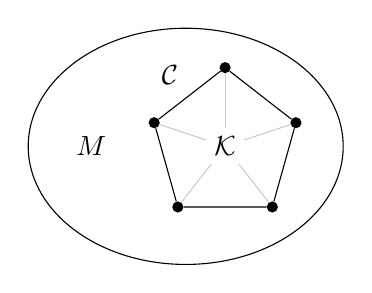
\begin{tikzpicture}
        \draw[fill=white] (-0.5, 0) ellipse (2cm and 1.5cm);
        %\draw[fill=lightgray, draw=black] (0,0) circle (1.25cm);
        %\draw[fill=white] (0,0) circle (0.75cm);
        \node at (-0.7, 0.9) {$\confg$};
        \node at (-1.7, 0) {$M$};

        \node[inner sep=1mm] (c) at (0, 0) {$\core$};
        \node[circle, fill, scale=0.015cm] (l1) at (0, 1) { };
        \node[circle, fill, scale=0.015cm] (l2) at (0.9, 0.30) { };
        \node[circle, fill, scale=0.015cm] (l3) at (0.6, -0.77) {};
        \node[circle, fill, scale=0.015cm] (l4) at (-0.6, -0.77) {};
        \node[circle, fill, scale=0.015cm] (l5) at (-0.9, 0.30) {};

        \draw[opacity=0.2] (c) -- (l1);
        \draw[opacity=0.2] (c) -- (l2);
        \draw[opacity=0.2] (c) -- (l3);
        \draw[opacity=0.2] (c) -- (l4);
        \draw[opacity=0.2] (c) -- (l5);
        \draw (l1) -- (l2) -- (l3) -- (l4) -- (l5) -- (l1);
    \end{tikzpicture}
    \caption{The graph $G=M + \confg$ that contains the configuration $\confg=R_5 + \core$.}
\end{figure}

The idea of $k$-reducibility is that we try to find a \textit{common ring coloring} for $M+R$ and the configuration $\core+R$. If two such colorings can be found, then we can combine both colorings to color $G$. This is exactly a more general approach to what we did for the five color theorem, where the configuration was the vertex $v$ with five neighbors.

Because we allow $M$ and $\confg$ to be arbitrary, we might not always be guaranteed to find a common ring coloring. To obtain certainty, we must have some control over the colorings on both sides. We can obtain this control by adding extra vertices on the other side of the ring in $M+R$ and $\core+R$. Consider the following two graphs.

\begin{figure}[!ht]
    \centering
    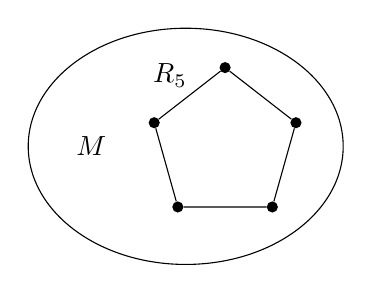
\begin{tikzpicture}
        \draw[fill=white] (-0.5, 0) ellipse (2cm and 1.5cm);
        \node at (-1.7, 0) {$M$};
        \node at (-0.7, 0.9) {$R_5$};

        \node[circle, fill, scale=0.015cm] (l1) at (0, 1) { };
        \node[circle, fill, scale=0.015cm] (l2) at (0.9, 0.30) { };
        \node[circle, fill, scale=0.015cm] (l3) at (0.6, -0.77) {};
        \node[circle, fill, scale=0.015cm] (l4) at (-0.6, -0.77) {};
        \node[circle, fill, scale=0.015cm] (l5) at (-0.9, 0.30) {};

        \draw (l1) -- (l2) -- (l3) -- (l4) -- (l5) -- (l1);
    \end{tikzpicture}
    \hspace{1cm}
    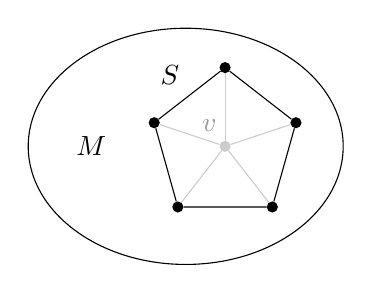
\begin{tikzpicture}
        \draw[fill=white] (-0.5, 0) ellipse (2cm and 1.5cm);
        \node at (-1.7, 0) {$M$};
        \node at (-0.7, 0.9) {$S$};

        \node[opacity=0.4] (c) at (-0.2, 0.27) { $v$ };
        \node[circle, fill, scale=0.015cm, opacity=0.2] (c) at (0, 0) {};
        \node[circle, fill, scale=0.015cm] (l1) at (0, 1) { };
        \node[circle, fill, scale=0.015cm] (l2) at (0.9, 0.30) { };
        \node[circle, fill, scale=0.015cm] (l3) at (0.6, -0.77) {};
        \node[circle, fill, scale=0.015cm] (l4) at (-0.6, -0.77) {};
        \node[circle, fill, scale=0.015cm] (l5) at (-0.9, 0.30) {};

        \draw[opacity=0.2] (c) -- (l1);
        \draw[opacity=0.2] (c) -- (l2);
        \draw[opacity=0.2] (c) -- (l3);
        \draw[opacity=0.2] (c) -- (l4);
        \draw[opacity=0.2] (c) -- (l5);
        \draw (l1) -- (l2) -- (l3) -- (l4) -- (l5) -- (l1);
    \end{tikzpicture}
    \caption{On the left, a graph $M+R_5$ without extra vertices. On the right, a graph $M+S$ where $S=R_5+v$. The graph $S$ is called a \textit{reducer}.}
    \label{fig:reducertut}
\end{figure}

The colorings of the ring in $M+R_5$ can be any 3-coloring or 4-coloring depending on $M$. However, in the graph $M+S$ it is not possible the color the ring in four colors. Due to the extra vertex introduced by $S$, we are guaranteed to find only 3-colorings on the ring regardless of $M$. An example of such a 3-coloring is $cabab$.

This guaranteed 3-coloring is key information in the reducibility proof of $R_5$. Therefore, let us instead reduce the graph $G=M+R+\core$ to

\begin{equation}
    M+S \;\;\text{and}\;\; \core+S' \quad \text{with} \quad R \subset S,S'.
\end{equation}

For both reducers $S$ and $S'$, we require that $|S-R| \leq k$. Here $k \geq 0$ is a limit on the amount of extra vertices we can add. Ideally, of course, we want $k=0$ such that we reduce the size of $G$ as much as possible. By increasing $k$, we get a smaller size reduction of $G$ in exchange for more control over the colorings.

\begin{itemize}
    \item If $k=0$, then $S=R$ and we reduce to $M_1+R$ and $\core+R$. This is the smallest possible reduction and ideal situation.
    \item If $k=1$, then we can set $S=R+v$ like in Figure \ref{fig:reducertut}. Our reduced graph is then one vertex larger.
    \item If $k = |\confg|$, then we can set $S = \confg$ and $S' = R$ such that we obtain $M+\confg$ and $\confg$. Clearly, they have a common ring coloring, but we did not achieve any reduction in size with $M+\confg = G$. 
\end{itemize}

Therefore, to obtain a reduction in size, we should also require that $k < |\confg|$. We are now ready to define this concept of reducibility.

\begin{definition}
    A configuration $\confg=\core+R$ is \emph{$k$-reducible} if for all planar graphs $G=M+\confg$ and some reducers $S$ and $S'$ on $\leq k < |\confg|$ vertices, there exists a common ring coloring for $M+S$ and $\core+S'$.
\end{definition}
\begin{definition}
    The ring $R_n$ is \emph{$k$-reducible} if all configurations $\confg$ on $R_n$ are at most $k$-reducible.
\end{definition}

A trivial example is the 0-reducibility of the rings $R_1, R_2$ and $R_3$. The only possible colorings on these rings are of the form $ a, ab$ and $ abc$ respectively. This means that any two colorings of $M+R$ and $\core + R$ are of this same form and therefore equal. You might say that the colorings $abab$ and $acac$ are different, but we can make them equal by renaming the color $b\rightarrow c$. We consider two colorings that have this property to be \textit{equal}.

\begin{definition}
    \label{def:coleq}
    Two colorings $x$ and $y$ are \emph{equal} if they differ only by a renaming of the colors $a,b,c$ and $d$. 
\end{definition}

Next, we move on to Kempe-chains.

\subsection{Kempe-chains}

Drawing again inspiration from the proof of the five color theorem. We had essentially proven that the vertex with five neighbors is a 0-reducible configuration. The key weapon we used in this proof was the notion of \textit{chains}. Therefore, we will try using them to prove general $k$-reducibility as well by giving a proper definition.

\begin{definition}
    Let $G_{ab}(x)$ be the subgraph consisting of all the vertices colored $ab$ in the coloring $x$ of $G$.
    Then the \emph{Kempe-chain} $\kappa_{ab}(v)$ or \emph{$ab$-chain} of the vertex $v$ is the component of $G_{ab}(x)$ that contains $v$. 
\end{definition}

\begin{figure}[!ht]
    \centering
    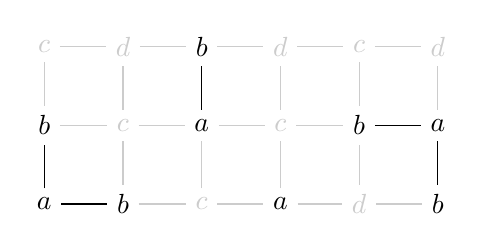
\begin{tikzpicture}[scale=1]
        \node (x11) at (0, 0) { $a$ };
        \node (x12) at (1, 0) { $b$ };
        \node[opacity=0.2] (x13) at (2, 0) { $c$ };
        \node (x21) at (0, 1) { $b$ };
        \node[opacity=0.2] (x22) at (1, 1) { $c$ };
        \node (x23) at (2, 1) { $a$ };
        \node[opacity=0.2] (x31) at (0, 2) { $c$ };
        \node[opacity=0.2] (x32) at (1, 2) { $d$ };
        \node (x33) at (2, 2) { $b$ };
        \node (y11) at (3, 0) { $a$ };
        \node[opacity=0.2] (y12) at (4, 0) { $d$ };
        \node (y13) at (5, 0) { $b$ };
        \node[opacity=0.2] (y21) at (3, 1) { $c$ };
        \node (y22) at (4, 1) { $b$ };
        \node (y23) at (5, 1) { $a$ };
        \node[opacity=0.2] (y31) at (3, 2) { $d$ };
        \node[opacity=0.2] (y32) at (4, 2) { $c$ };
        \node[opacity=0.2] (y33) at (5, 2) { $d$ };

        \draw (x11) -- (x12);
        \draw[opacity=0.2] (x12) -- (x13);

        \draw[opacity=0.2] (x21) -- (x22);
        \draw[opacity=0.2] (x22) -- (x23);
        \draw[opacity=0.2] (x31) -- (x32);
        \draw[opacity=0.2] (x32) -- (x33);

        \draw (x11) -- (x21);
        \draw[opacity=0.2] (x21) -- (x31);
        \draw[opacity=0.2] (x12) -- (x22) -- (x32);
        \draw[opacity=0.2] (x13) -- (x23);
        \draw (x23) -- (x33);

        \draw[opacity=0.2] (y11) -- (y12) -- (y13);
        \draw[opacity=0.2] (y21) -- (y22);
        \draw (y22) -- (y23);
        \draw[opacity=0.2] (y31) -- (y32) -- (y33);

        \draw[opacity=0.2] (y11) -- (y21) -- (y31);
        \draw[opacity=0.2] (y12) -- (y22) -- (y32);
        \draw (y13) -- (y23);
        \draw[opacity=0.2] (y23) -- (y33);

        \draw[opacity=0.2] (x13) -- (y11);
        \draw[opacity=0.2] (x23) -- (y21);
        \draw[opacity=0.2] (x33) -- (y31);
    \end{tikzpicture}
    \caption{The components of $G_{ab}(x)$ for a planar graph $G$ and its coloring $x$ are highlighted. We write $\chain{u}{v}{ab}$ or $u \in \kappa_{ab}(v)$ if $u$ and $v$ are on the same component.}
    \label{fig:kempetut}
\end{figure}

As we have seen before, we can flip the colors of a chain $\kappa_{ab}(v)$ without breaking the current coloring. Imagine in your head how you can swap the chains in Figure \ref{fig:kempetut} for example. This key property of chains will allow us to obtain new ring colorings.

Judging only from the colors of a ring such as in $abcab$, we have no information on the chains that are present. This information is important because two vertices of the ring that belong to the same chain must be flipped together.

To include this information in a ring coloring, Birkhoff devised the notion of a \textit{scheme}. He simply draws a line between two colors on the ring if they belong to the same Kempe-chain.

\begin{definition}
    Given a coloring $x$ of a planar graph $G$ and the colors on its ring $x(R)$. The \emph{scheme} on $R$ of $x$ consists of $x(R)$ with knowledge whether $u \in \kappa_{ab}(v)$ for two ring vertices $u,v \in R$ and colors $ab$.
\end{definition}
\begin{figure}[!ht]
    \centering
    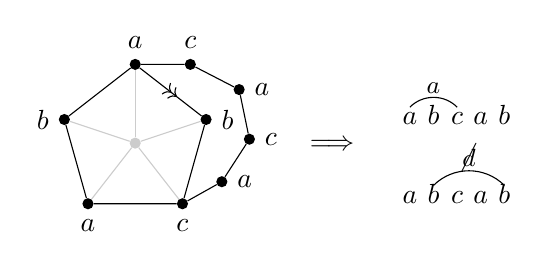
\begin{tikzpicture}[scale=1.0, mid arrow/.style={
        postaction={ decorate, decoration={ markings, mark=at position 0.6 with { \arrow[black]{>>} } } } }]

        \node[circle, fill, scale=0.015cm, opacity=0.2] (v) at (0, 0) { };
        \node[circle, fill, scale=0.015cm, label=above:$a$] (l1) at (0, 1) { };
        \node[circle, fill, scale=0.015cm, label=right:$b$] (l2) at (0.9, 0.30) { };
        \node[circle, fill, scale=0.015cm, label=below:$c$] (l3) at (0.6, -0.77) {};
        \node[circle, fill, scale=0.015cm, label=below:$a$] (l4) at (-0.6, -0.77) {};
        \node[circle, fill, scale=0.015cm, label=left:$b$] (l5) at (-0.9, 0.30) {};
        \node[circle, fill, scale=0.015cm, label=above:$c$] (c1) at (0.7, 1) {};
        \node[circle, fill, scale=0.015cm, label=right:$a$] (c2) at (1.32, 0.68) {};
        \node[circle, fill, scale=0.015cm, label=right:$c$] (c3) at (1.45, 0.05) {};
        \node[circle, fill, scale=0.015cm, label=right:$a$] (c4) at (1.1, -0.49) {};
        \draw[mid arrow] (l1) -- (l2);
        \draw (l2) -- (l3) -- (l4) -- (l5) -- (l1);
        \draw (l1) -- (c1) -- (c2) -- (c3) -- (c4) -- (l3);
        \draw[opacity=0.2] (l1) -- (v);
        \draw[opacity=0.2] (l2) -- (v);
        \draw[opacity=0.2] (l3) -- (v);
        \draw[opacity=0.2] (l4) -- (v); 
        \draw[opacity=0.2] (l5) -- (v);
        \node (impl) at (3, 0) { $\hspace{1cm} \implies \hspace{0.3cm} \begin{matrix}
            \scheme{a,b,c,a,b}{ 13a } \\
            \scheme{a,b,c,a,b}{ 25d- }
        \end{matrix}$ };
        
    \end{tikzpicture}
    \caption{Two ring schemes that are derived from a graph coloring. We only consider the chains on one side of the ring. The strikethrough $\cancel{d}$ indicates absence of a chain. Refer to the main.tex file \cite{github} for the \;\LaTeX\; source of this notation. }
    \label{fig:schemes}
\end{figure}

A coloring can be treated as a scheme without information on chains. A scheme can be treated as a coloring. As such, we will use them interchangeably from now on. 

Given the information of Kempe-chains on a coloring, we can start modifying the colors of the ring by flipping chains. We call any coloring that can be derived in this manner an \textit{implied coloring} of the scheme. 

\begin{definition}
    Given two schemes $x$ and $y$. We say that $x$ implies $y$ if $x=y$ or $y$ can be obtained from $x$ by flipping a Kempe-chain. Write $x\compat y$.
\end{definition}

For example, the two schemes from Figure \ref{fig:schemes} have the following implications (change is highlighted).

\begin{equation*}
    \scheme{a,b,c,a,b}{ 13a } \compat \scheme{a,b,c,a,\textbf{d}}{{13a}}, \quad \quad
    \scheme{a,b,c,a,b}{ 25d- } \compat \scheme{a,\textbf{d},c,a,b}{{25d-}}.
\end{equation*}

We have now built a strong theory to modify ring colorings using schemes and Kempe-chains, all inspired by the proof of the five color theorem. You can try for yourself to rewrite that proof using scheme notation (assume that the neighbors form a ring). With these tools, we are now ready to prove the $k$-reducibility of rings.
\subsection{0-reducibility of the ring $R_4$}

We will show that all configurations on the ring $R_4$ are reducible without the need for a reducer. This proof and the proof of the five color theorem are very much alike.

\begin{theorem}
    The ring $R_4$ is 0-reducible.
\end{theorem}
\begin{proof}

Let the planar graph $M+\confg$ with configuration $\confg = \core + R_4$ be arbitrary. Since we set $k=0$, we will try reducing to $M+R_4$ and $\confg$. For convenience, let the possible ring colorings of these two reductions be represented by the sets

\begin{equation}
    \I = \Phi(M+R_4) \quad \text{and} \quad \II = \Phi(\confg).
\end{equation}

To gain an insight into the possible colorings of these sets, we sketched the situation in Figure \ref{fig:ring4tut}.

\begin{figure}[!ht]
    \centering
    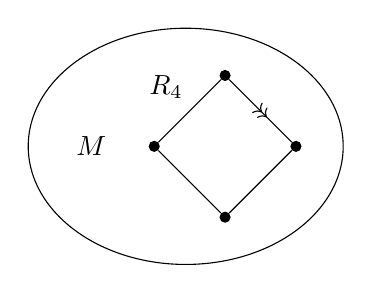
\begin{tikzpicture}[mid arrow/.style={
        postaction={ decorate, decoration={ markings, mark=at position 0.6 with { \arrow[black]{>>} } } } }]
        \draw[fill=white] (-0.5, 0) ellipse (2cm and 1.5cm);
        \node (m) at (-1.7, 0) {$M$};
        \node at (-0.75, 0.75) {$R_4$};

        \node[circle, fill, scale=0.015cm] (l1) at (0, 0.9) { };
        \node[circle, fill, scale=0.015cm] (l2) at (0.9, 0) { };
        \node[circle, fill, scale=0.015cm] (l3) at (0, -0.9) {};
        \node[circle, fill, scale=0.015cm] (l4) at (-0.9, 0) {};

        \draw[mid arrow] (l1) -- (l2);
        \draw (l2) -- (l3) -- (l4) -- (l1);
    \end{tikzpicture}
    \begin{tikzpicture}[mid arrow/.style={
        postaction={ decorate, decoration={ markings, mark=at position 0.6 with { \arrow[black]{>>} } } } }]
        \draw[opacity=0] (-0.5, 0) ellipse (2cm and 1.5cm);
        \node at (-0.75, 0.75) {$R_4$};
        \node[inner sep=1mm] (c) at (0, 0) {$\core$};

        \node[circle, fill, scale=0.015cm] (l1) at (0, 0.9) { };
        \node[circle, fill, scale=0.015cm] (l2) at (0.9, 0) { };
        \node[circle, fill, scale=0.015cm] (l3) at (0, -0.9) {};
        \node[circle, fill, scale=0.015cm] (l4) at (-0.9, 0) {};

        \draw[mid arrow] (l1) -- (l2);
        \draw (l2) -- (l3) -- (l4) -- (l1);
        \draw[opacity=0.2] (l1) -- (c);
        \draw[opacity=0.2] (l2) -- (c); 
        \draw[opacity=0.2] (l3) -- (c);
        \draw[opacity=0.2] (l4) -- (c);
    \end{tikzpicture}
    \caption{The reductions $M+R_4$ and $\core+R_4$ ($\confg$). What can we say about their possible ring colorings $\I$ and $\II$?}
    \label{fig:ring4tut}
\end{figure}

You might have noticed that both reductions contain the plain ring $R_4$ with no other vertices on one side. Therefore, as we have shown in Theorem \ref{thm:ringsarered} about plain ring reducibility, we may contract any two non-neighboring vertices to obtain further reductions.

We wont sketch these contracted graphs here, but in the context of ring colorings in $\I$ and $\II$, we will obtain colorings of $R_4$ with two contracted vertices colored the same. Because there are two ways to contract vertices on $R_4$ (the two diagonals), we are guaranteed of the following two colorings in $\I$ and $\II$.

\begin{equation}
    \left\{\begin{matrix}
        abab \;\;\text{or}\;\; abac, \\
        baba \;\;\text{or}\;\; baca
    \end{matrix}\right\} \subset I,II.
\end{equation}

Let us evaluate every pair of possibilities to see if there is a common coloring. First note that $abab=baba$ by definition of equality between ring colorings (Definition \ref{def:coleq}). Then, there remain 3 possible sets for $\I$ and $\II$.

\needspace{2cm}
\begin{equation}
    \circled{1} = \{ abab \}, \quad \circled{2} = \left\{ \begin{matrix}abab \\ baca\end{matrix} \right\}, \quad \circled{3} = \left\{ \begin{matrix}abac \\ baca \end{matrix} \right\}.
\end{equation}

You might already see that there is only one pair where we must actually show something, because
\begin{enumerate}
    \item $\I = \circled{1}$ and $\II = \circled{2}$ implies that $abab$ is the common coloring.
    \item $\I = \circled{2}$ and $\II = \circled{3}$ implies that $baca$ is the common coloring.
    \item $\I = \circled{1}$ and $\II = \circled{3}$. This is where Kempe-chains come in.
\end{enumerate}

To handle the third case, let $\I = \{ abab \}$ and $\II = \{ abac, baca \}$. Similar to what we did with the five color theorem, suppose that in the coloring $\I(abab)$ we have $\chain{v_1}{v_3}{ad}$. In both cases we obtain

\begin{equation}
    \begin{aligned}
        \I(abab) &= \scheme{a,b,a,b}{13d} \compat \II(abac) \\
        \I(abab) &= \scheme{a,b,a,b}{13d-} \compat \I(abcb) = \II(baca).
    \end{aligned}
\end{equation}

In any case, we obtain a common ring coloring between $\I$ and $\II$. Therefore the ring $R_4$ is 0-reducible.
\end{proof}
\subsection{1-reducibility of the ring $R_5$}

In the five color theorem, we used that every planar graph has a vertex with $\deg(v)\leq 5$. So far, we know that the cases $\deg(v) \leq 4$ are reducible when using four colors. If $\deg(v)=5$, we may add edges between the neighbors of $v$ to obtain the ring $R_5$. If $R_5$ were 0-reducible, then we would obtain our reduction by removing the vertex $v$. Therefore, the four color theorem would follow in the same fashion as the five color theorem.

Many have tried to show this, among which Alfred Kempe with his false proof. It must be hard (or require clever tricks) to prove that $R_5$ is 0-reducible. That is why Birhoff had proven in 1913 that $R_5$ is 1-reducible instead \cite{birkhoff}. So will we.

\begin{theorem}
    The ring $R_5$ is 1-reducible.
\end{theorem}

\begin{proof}
Let the planar graph $M+\confg$ with configuration $\confg=\core+R_5$ be arbitrary. Again, let the possible ring colorings be represented by

\begin{equation}
    \I = \Phi(M+S) \quad \text{and} \quad \II = \Phi(\core+S').
\end{equation}

Since $k=1$, we have colorings from both $S=R_5$ and $S=R_5+v$ in the sets of possible colorings $\I, \II$. Whether or not we need the reducer depends totally on the arbitrary choice of $M+\confg$. This is as expected, since there are many configurations that are in fact, 0-reducible.

Let us first consider the colorings contributed by the choice $S=R_5$, which means that we dont use a reducer.

\begin{figure}[!ht] 
    \centering
    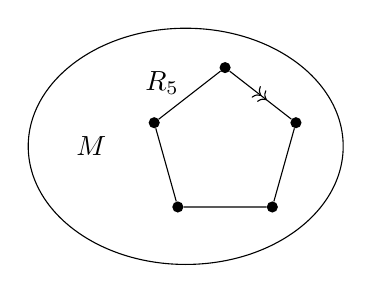
\begin{tikzpicture}[mid arrow/.style={
        postaction={ decorate, decoration={ markings, mark=at position 0.6 with { \arrow[black]{>>} } } } }]
        \draw[fill=white] (-0.5, 0) ellipse (2cm and 1.5cm);
        \node (m) at (-1.7, 0) {$M$};
        \node at (-0.8, 0.8) {$R_5$};

        \node[circle, fill, scale=0.015cm] (l1) at (0, 1) { };
        \node[circle, fill, scale=0.015cm] (l2) at (0.9, 0.30) { };
        \node[circle, fill, scale=0.015cm] (l3) at (0.6, -0.77) {};
        \node[circle, fill, scale=0.015cm] (l4) at (-0.6, -0.77) {};
        \node[circle, fill, scale=0.015cm] (l5) at (-0.9, 0.30) {};
        \draw[mid arrow] (l1) -- (l2);
        \draw (l2) -- (l3) -- (l4) -- (l5) -- (l1);
    \end{tikzpicture}
    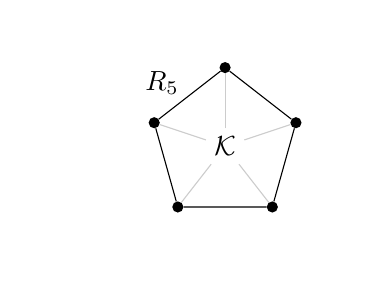
\begin{tikzpicture}[mid arrow/.style={
        postaction={ decorate, decoration={ markings, mark=at position 0.6 with { \arrow[black]{>>} } } } }]
        \draw[opacity=0] (-0.5, 0) ellipse (2cm and 1.5cm);
        \node at (-0.8, 0.8) {$R_5$};
        \node[inner sep=1mm] (c) at (0, 0) {$\core$};
        \node[circle, fill, scale=0.015cm] (l1) at (0, 1) { };
        \node[circle, fill, scale=0.015cm] (l2) at (0.9, 0.30) { };
        \node[circle, fill, scale=0.015cm] (l3) at (0.6, -0.77) {};
        \node[circle, fill, scale=0.015cm] (l4) at (-0.6, -0.77) {};
        \node[circle, fill, scale=0.015cm] (l5) at (-0.9, 0.30) {};

        \draw[opacity=0.2] (c) -- (l1);
        \draw[opacity=0.2] (c) -- (l2);
        \draw[opacity=0.2] (c) -- (l3);
        \draw[opacity=0.2] (c) -- (l4);
        \draw[opacity=0.2] (c) -- (l5);
        \draw (l1) -- (l2) -- (l3) -- (l4) -- (l5) -- (l1);
    \end{tikzpicture}
    \caption{The reductions $M+R_5$ and $\core+R_5$ ($\confg$).}
    \label{fig:ring5k0}
\end{figure}

Now we use the same trick as for the ring $R_4$. We may contract any two non-neighboring vertices of $R_5$ by Theorem \ref{thm:ringsarered}. This means that we get colorings of the form $a{*}{*}a{*}$ where the $a$-colored vertices got contracted. We dont know anything about the ${*}$-colors. Since there are 5 possible contractions of two vertices on $R_5$, we obtain 5 different colorings.

\begin{equation}
    \Phi^\star = \{ a{*}{*}a{*}, \quad {*}a{*}{*}a, \quad a{*}a{*}{*}, \quad {*}a{*}a{*}, \quad {*}{*}a{*}a{*} \}.
\end{equation}

Next we consider the colorings for $S=R_5+v$. We may freely choose our reducers $S$ and $S'$ here. We will try to guarantee a 3-coloring because they are simplest to work with. It also turns out that they are key to finding a common ring coloring, as we shall see. For this reason, we use a single vertex connected to all ring vertices for our reducers $S$ and $S'$. 

Note that the ${*}$-colorings from $\Phi^\star$ dont guarantee a 3-coloring. You can see how trying to prove 0-reducibility ($k=0$) requires you to work only with these colorings, and hence without a guarantee on any kind of coloring. A lot of cases will have to be evaluated.

\needspace{5cm}
\begin{figure}[!ht]
    \centering
    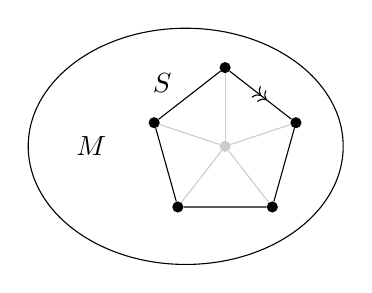
\begin{tikzpicture}[mid arrow/.style={
        postaction={ decorate, decoration={ markings, mark=at position 0.6 with { \arrow[black]{>>} } } } }]
        \draw[fill=white] (-0.5, 0) ellipse (2cm and 1.5cm);
        \node (m) at (-1.7, 0) {$M$};
        \node at (-0.8, 0.8) {$S$};

        \node[circle, fill, scale=0.015cm] (l1) at (0, 1) { };
        \node[circle, fill, scale=0.015cm] (l2) at (0.9, 0.30) { };
        \node[circle, fill, scale=0.015cm] (l3) at (0.6, -0.77) {};
        \node[circle, fill, scale=0.015cm] (l4) at (-0.6, -0.77) {};
        \node[circle, fill, scale=0.015cm] (l5) at (-0.9, 0.30) {};
        \node[circle, fill, scale=0.015cm, opacity=0.2] (e) at (0, 0) { };

        \draw[opacity=0.2] (e) -- (l1);
        \draw[opacity=0.2] (e) -- (l2);
        \draw[opacity=0.2] (e) -- (l3);
        \draw[opacity=0.2] (e) -- (l4);
        \draw[opacity=0.2] (e) -- (l5);
        \draw[mid arrow] (l1) -- (l2);
        \draw (l2) -- (l3) -- (l4) -- (l5) -- (l1);
    \end{tikzpicture}
    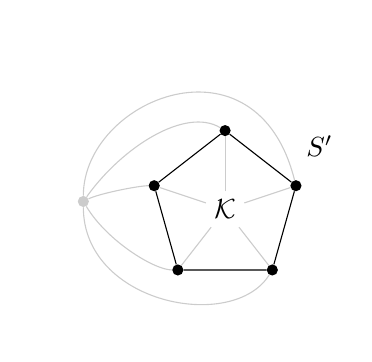
\begin{tikzpicture}[mid arrow/.style={
        postaction={ decorate, decoration={ markings, mark=at position 0.6 with { \arrow[black]{>>} } } } }]
        \draw[opacity=0] (-0.5, 0) ellipse (2cm and 1.5cm);
        \node[fill=white] at (1.2, 0.8) {$S'$};
        \node[inner sep=1mm] (c) at (0, 0) {$\core$};
        \node[circle, fill, scale=0.015cm] (l1) at (0, 1) { };
        \node[circle, fill, scale=0.015cm] (l2) at (0.9, 0.30) { };
        \node[circle, fill, scale=0.015cm] (l3) at (0.6, -0.77) {};
        \node[circle, fill, scale=0.015cm] (l4) at (-0.6, -0.77) {};
        \node[circle, fill, scale=0.015cm] (l5) at (-0.9, 0.30) {};
        \node[circle, fill, scale=0.015cm, opacity=0.2] (e) at (-1.8, 0.1) { };

        \draw[opacity=0.2] (e) .. controls +(0.2, 0.1) and + (-0.2, 0.0) .. (l5);
        \draw[opacity=0.2] (e) .. controls +(0.3, -0.5) and +(-0.3,0) .. (l4);
        \draw[opacity=0.2] (e) .. controls +(0.0,-1.3) and +(-0.5,-0.8) .. (l3);
        \draw[opacity=0.2] (e) .. controls +(0.0,+1.3) and +(-0.5,+2) .. (l2);
        \draw[opacity=0.2] (e) .. controls +(0.5,0.7) and +(-0.5, 0.3) .. (l1);

        \draw[opacity=0.2] (c) -- (l1);
        \draw[opacity=0.2] (c) -- (l2);
        \draw[opacity=0.2] (c) -- (l3);
        \draw[opacity=0.2] (c) -- (l4);
        \draw[opacity=0.2] (c) -- (l5);
        \draw (l1) -- (l2) -- (l3) -- (l4) -- (l5) -- (l1);
    \end{tikzpicture}
    \caption{The reductions $M+S$ and $\core+S'$ with $S=R_5+v$ for our specific choice of $S$ and $S'$.  }
    \label{fig:ring5k1}
\end{figure}

As expected, the only possible colorings of these reductions are 3-colorings like $\underline{c}abab$. There are five different 3-colorings of the ring $R_5$, we will be guaranteed of only one of them.

\begin{equation}
    \Phi^S = \{ 
        \underline{c}abab\;\;\text{or}\;\; 
        a\underline{c}bab\;\;\text{or}\;\;
        ab\underline{c}ab\;\;\text{or}\;\;
        aba\underline{c}b\;\;\text{or}\;\;
        abab\underline{c} \}.
\end{equation}

Taking everything together, we obtain the following guarantee on colorings in $\I$ and $\II$.

\begin{equation}
    \Phi^\star\; \cup \;\Phi^S \;\subset\; \I, \II.
\end{equation}

A special property of 3-colorings on $R_5$ is that there will always be a single vertex colored uniquely, we call this the \textit{marked vertex}. This vertex acts as a kind of 'pivot' to tell if two 3-colorings are \textit{adjacent}. These two concepts are key to the proof.

\begin{definition}
    The uniquely-colored vertex of a 3-coloring of $R_5$ is called the \emph{marked vertex}, indicated by an underline such as in $\underline{c}abab$.
\end{definition}

\begin{definition}
    Two 3-colorings of $R_5$ are called \emph{adjacent} if they have adjacent marked vertices, such as in $\underline{c}abab$ and $a\underline{c}bab$.
\end{definition}

Since we have guaranteed 3-colorings for both $\I$ and $\II$, we can split up our proof into 3 cases.

\begin{enumerate}
    \item $\I$ and $\II$ have an adjacent coloring ($\underline{c}abab$ and $a\underline{c}bab$).
    \item $\I$ and $\II$ have a non-adjacent coloring ($\underline{c}abab$ and $ab\underline{c}ab$).
    \item $\I$ and $\II$ have a coloring with the same marked vertex ($\underline{c}abab$ and $\underline{d}cbcb$). This always results in a common coloring.
\end{enumerate}

Therefore, we only need to consider the cases \circled{1} and \circled{2}. We will prove two lemma's to this end. Their relation is illustrated below.

\begin{equation*}
    \begin{aligned}
    \circled{2} \implies\; &\circled{1}\quad \text{or} \quad \text{common coloring} \quad\quad \text{(Lemma \ref{lem:r5_first})} \\
    &\downarrow \\
    &\circled{1} \implies\;\text{common coloring}\quad\quad \text{(Lemma \ref{lem:r5_second})}
    \end{aligned}
\end{equation*}

\begin{lemma}
    \label{lem:r5_first}
    If $\I$ and $\II$ have a non-adjacent coloring, then they either have an adjacent coloring or a common coloring.
\end{lemma}

\begin{proof}
Let two non-adjacent colorings $\I(\underline{c}abab)$ and $\II(ab\underline{c}ab)$ be given. Suppose that $v_3 \stackrel{bc}{\frown} v_5$ in $\II(ab\underline{c}ab)$. The two cases lead to the following.

\begin{equation}
    \label{eq:abcab}
    \begin{aligned}
        \II(ab\underline{c}ab) &=\scheme{a,b,c,a,b}{35b} \compat \II(abcdb), \\
        \II(ab\underline{c}ab) &= \scheme{a,b,c,a,b}{35b-} \compat \II(a\underline{c}bab).
    \end{aligned}
\end{equation}

The second case results in a coloring adjacent to $\I(\underline{c}abab)$. For the first case, we consider the coloring $\I({*}b{*}{*}b)$. The two adjacent ${*}$-colors must be different from each other and $b$, therefore we may assume that we have $\I({*}bcdb)$. The last ${*}$-color reveals 3 possibilities.

\begin{equation}
    \begin{matrix*}[l]
        \I(abcdb) \quad\quad =&\II(abcdb) \; \text{from (\ref{eq:abcab}),}  \\
        \I(cbc\underline{d}b) \;\; \text{adjacent to}&\II(ab\underline{c}ab), \;  \\
        \I(db\underline{c}db) \quad\quad =&\II(ab\underline{c}ab).
    \end{matrix*}
\end{equation}

Therefore we obtain either a common coloring or an adjacent coloring. Note that the pair of non-adjacent colorings we chose is the only unique one on $R_5$ (up to rotational symmetry).
\end{proof}

\begin{lemma}
    \label{lem:r5_second}
    If I and II have an adjacent coloring, then they have a common coloring.
\end{lemma}

\begin{proof}

Let two adjacent colorings $\I(\underline{c}abab)$ and $\II(a\underline{c}bab)$ be given. Suppose that $\chain{v_3}{v_5}{bd}$ in $\II(a\underline{c}bab)$. The two cases lead to the following.

\begin{equation}
    \label{eq:acdab}
    \begin{aligned}
        \II(a\underline{c}bab) &= \scheme{a,c,b,a,b}{35d} \compat \I(\underline{c}abab). \\
        \II(a\underline{c}bab) &= \scheme{a,c,b,a,b}{35d-} \compat \II(acdab).
    \end{aligned}
\end{equation}

The first case leads to a common coloring. For the second case,
we consider the coloring $\I(a{*}{*}a{*})$. We may again assume to have $\I(acda{*})$. Then the 3 remaining possibilities for the ${*}$-color are

\begin{equation*}
    \begin{matrix*}[l]
        \I(acdab) \quad =& \II(acdab), \;\text{from (\ref{eq:acdab})},\\
        \I(ac\underline{d}ac) \quad =\;\; \text{shifted $+2$}& \I(\underline{c}abab), \\
        \I(a\underline{c}dad) \quad =& \II(a\underline{c}bab).
    \end{matrix*}
\end{equation*}

If we do not obtain common colorings, we may repeat this procedure with $\II(a\underline{c}bab)$ and $\I(ac\underline{d}ac)$ to continously shift the marked vertex two to the right. The pattern that arises is illustrated in Figure \ref{table:ringpattern5} below.

\begin{figure}[!ht]
    \centering
    \begin{tabular}{c|ccccc:c}
         & $v_1$ & $v_2$  & $v_3$  & $v_4$ & $v_5$ & $v_1$  \\
        \hline
        1 & \I & \II &    &     &    & \I  \\
        2 &    & \II & \I &     &    &     \\
        3 &    &     & \I & \II &    &     \\
        4 &    &     &    & \II & \I &     \\
        5 &    &     &    &     & \I & \II \\
    \end{tabular}
    \caption{Marked vertices of $\I$ and $\II$ obtained by repetition of the earlier procedure.  Every step shifts the leftmost marked vertex two to the right. }
    \label{table:ringpattern5}
\end{figure}

At iteration 5, we obtain that $\II$ has the same marked vertex $v_1$ as $\I$. Therefore, by repetition we obtain that

\begin{equation}
    \II(\underline{c}abab) \rightarrow \II(aba\underline{c}b) \rightarrow \II(\underline{c}abab) = \I(\underline{c}abab).
\end{equation}

Therefore, adjacent colorings imply a common coloring for $\I$ and $\II$.

\end{proof}

Combining these two lemmas yields a guaranteed common ring coloring for $\I$ and $\II$ regardless of the case.

\end{proof}

In practice, the first step is to find the guaranteed 3-colorings from $M+S$ and $\core+S'$. Then, by conditioning on the marked vertex, we may need to use up to two ${*}$-colorings ($M$ and $\confg$ one each) depending on the Kempe-chains in the 3-colorings. Each ${*}$-coloring corresponds to a contraction of the ring vertices in $M+R_5$ or $\core+R_5$. Therefore, in the worst case, we have to color 4 smaller graphs before we can color $M+\confg$. In the ideal case only 2.
\section{D-Reducibility}
\label{sec:dreduce}

We have seen that the ring $R_4$ is 0-reducible and the that the ring $R_5$ is 1-reducible. This essentially provides us with an two infinite classes of reducible configurations. However, it is not yet guaranteed that every planar graph contains such a $k$-reducible configuration on $R_4$ or $R_5$. Therefore, we must still look for more reducible configurations.

Naturally, we might try to examine the $k$-reducibility of $R_6$ and beyond. However, as we have seen in the increase in complexity for the 1-reducibility of $R_5$, this is a very tough problem. There are much more cases to consider for the ring $R_6$ than for $R_4$ and $R_5$. However, the difficulty of $k$-reducibility lies in the fact the we try to prove the reducibility of \textit{all} configurations $\confg$ on $R_n$ at once. Individual configurations are much easier to examine. 

Let us introduce the idea of D-reducibility, by working with an example. The very first, smallest and most famous configuration used in the proof of the four color theorem is the \textit{Birkhoff Diamond}  ($\text{Bir}\Diamond$). It is a configuration on $R_6$ with 4 vertices in the core.

\begin{figure}[!ht]
    \centering
    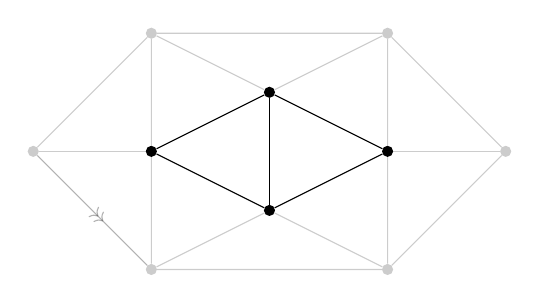
\begin{tikzpicture}[scale=1.5, mid arrow/.style={
        postaction={ decorate, decoration={ markings, mark=at position 0.6 with { \arrow[black]{>>} } } } }]
        \node[circle, fill, scale=0.015cm, opacity=0.2] (l1) at (-2, 0) { };
        \node[circle, fill, scale=0.015cm, opacity=0.2] (l2) at (-1, 1) { };
        \node[circle, fill, scale=0.015cm] (l3) at (-1, 0) {};
        \node[circle, fill, scale=0.015cm, opacity=0.2] (l4) at (-1, -1) {};

        \node[circle, fill, scale=0.015cm, opacity=0.2] (r1) at (2, 0) {};
        \node[circle, fill, scale=0.015cm, opacity=0.2] (r2) at (1, 1) {};
        \node[circle, fill, scale=0.015cm] (r3) at (1, 0) {};
        \node[circle, fill, scale=0.015cm, opacity=0.2] (r4) at (1, -1) {};

        \node[circle, fill, scale=0.015cm] (c1) at (0, 0.5) {};
        \node[circle, fill, scale=0.015cm] (c2) at (0, -0.5) {};

        \draw[opacity=0.2] (l1) -- (l2) -- (r2) -- (r1) -- (r4) -- (l4);
        \draw [mid arrow, opacity=0.3] (l1) -- (l4);
        \draw[opacity=0.2] (l1) -- (l3);
        \draw[opacity=0.2] (l2) -- (l3) -- (l4);
        \draw[opacity=0.2] (l2) -- (c1);
        \draw (c1) -- (l3) -- (c2);
        \draw[opacity=0.2] (c2) -- (l4);
        \draw (c1) -- (c2);
        \draw[opacity=0.2] (r2) -- (c1);
        \draw (c1) -- (r3) -- (c2);
        \draw[opacity=0.2] (c2) -- (r4);
        \draw[opacity=0.2] (r2) -- (r3) -- (r4);
        \draw[opacity=0.2] (r1) -- (r3);
    \end{tikzpicture}
    \caption{The Birkhoff Diamond $\confg = \bir$ with the core highlighted. }
    \label{fig:diamond}
\end{figure}

We highlighted the core $\core$ of the Birkhoff Diamond here, to explain the format of the \textit{unavoidable set of reducible configurations} found in the original proofs. Every (triangular) configuration with a ring is uniquely determined by its core $\core$ and the amount of edges that a vertex of the core $\core$ has in $\confg$.

For example, the Birkhoff Diamond is uniquely determined by the four vertices in the middle and the requirement that $\deg_\confg(v) = 5$ for each vertex in the core. To save space when storing configuations on paper or digitally, only this information of the core is actually needed.

We will show that $\bir$ is 0-reducible. Since we know the graph of $\bir$, we can write down all the colorings it can have on the ring. This is the set $\Phi(\bir)$ of 16 colorings. See Figure \ref{table:diamondphi0}.

\needspace{2cm}
\begin{figure}[!ht]
    \centering
    \begin{tabular}{ cccc }
        $\Phi(\bir) $ & \\
        \hline
        ababac & abacdb & abcadb & abcbcd \\
        ababcb & abacdc & abcbab & abcdab \\ 
        abacac & abcacb & abcbac & abcdcb \\
        abacbc & abcacd & abcbad & abcdcd \\
        \hline
        16 & \\
    \end{tabular}
    \caption{The unique ring colorings of $\bir$.}
    \label{table:diamondphi0}
\end{figure}

\needspace{1cm}
Therefore, if we want that $\bir$ is 0-reducible, we must show that any ring coloring of $M+R_6$ falls in the set $\Phi(\bir)$. When we were working with rings, we could only use the set of \textit{guaranteed} colorings of $\confg$. However, with an actual configuration like $\bir$, we know exactly which colorings are present. So we have much more control and precision to prove 0-reducibility.

If we let $M+R_6$ be arbitrary, then we can expect any ring coloring of $R_6$. Thus we must show that every coloring of $\Phi(6)$ can be changed to a coloring of $\Phi(\bir)$. The set $\Phi(6)$ can be seen in Figure \ref{table:colsring6}.

\begin{figure}[!ht]
    \centering
    \begin{tabular}{ cccc }
        $\Phi(6) $ & \\
        \hline
        ababab & abacbd & abcadc &  \cellcolor{g0} abcdab \\
        \cellcolor{g0} ababac &  \cellcolor{g0} abacdb &  \cellcolor{g0} abcbab & abcdac \\
        \cellcolor{g0} ababcb &  \cellcolor{g0} abacdc &  \cellcolor{g0} abcbac & abcdad \\
        ababcd & abcabc &  \cellcolor{g0} abcbad & abcdbc \\
        abacab & abcabd & abcbcb & abcdbd \\
        \cellcolor{g0} abacac &  \cellcolor{g0} abcacb &  \cellcolor{g0} abcbcd &  \cellcolor{g0} abcdcb \\
        abacad &  \cellcolor{g0} abcacd & abcbdb &  \cellcolor{g0} abcdcd \\
        \cellcolor{g0} abacbc &  \cellcolor{g0} abcadb & abcbdc \\
        \hline
        31 & \\
    \end{tabular}
    \caption{All unique ring colorings of $R_6$. The colorings of $\Phi(\bir)$ are highlighted. }
    \label{table:colsring6}
\end{figure}

As you can see, roughly half of the colorings is not directly compatible with $\bir$. Similar to what we did for the 1-reducibility of $R_5$, we will use Kempe-chains to change incompatible colorings to colorings in $\Phi(\bir)$.

Let us consider the coloring $ababab$ for example. Suppose that $\chain{v_4}{v_6}{bd}$. This implies the following colorings.

\begin{equation}
    \begin{aligned}
    \scheme{a,b,a,b,a,b}{46d} &\compat ababcb\\
    \scheme{a,b,a,b,a,b}{46d-} &\compat ababad = ababac.
    \end{aligned}
\end{equation}

Therefore, the coloring $ababab$ can be turned into a compatible coloring with only one chain flip. We say that the coloring $ababab$ \textit{implies} the set of colorings 

\begin{equation}
    ababab \compat \{ ababcb, ababac \}.
\end{equation}

This idea of a coloring implying a set of other colorings lies at the heart of D-reducibility, hence we will define it.

\begin{definition}
    A coloring $x$ implies a set of colorings $\II$ if every scheme $x^\star$ of $x$ implies a coloring $y \in \II$. Write $x \compat \II$.
\end{definition}

\begin{definition}
    A set of colorings $\I$ implies $\II$ if every $x \in \I$ implies $\II$. Write $\I \implies \II$.
\end{definition}

Now, let us find all the colorings of $R_6$ that require one chain flip to become compatible in the same way as $ababab$. This set is called the 1-implying set of $\bir$.

\begin{figure}[!ht]
    \centering
    \begin{tabular}{ cc }
        $\Phi_1(\bir) $ \\
        \hline
        ababab & abcbcb \\
        ababcd & abcdad\\
        abacab \\
        \hline
        5 \\
    \end{tabular}
    \caption{The 1-implying set $\Phi_1(\bir)$.}
    \label{table:diamondphi1}
\end{figure}

This is the largest set that satisfies $\Phi_1(\bir) \compat \Phi(\bir)$. We may repeat what we did for $\Phi_1(\bir)$ to obtain sets of colorings that require 2, 3 and more chain flips to become a coloring in $\Phi(\bir)$.

\begin{equation}
    \Phi_5(\bir) \compat \Phi_4(\bir) \compat \Phi_3(\bir) \compat \ldots \compat \Phi(\bir).
\end{equation}

Let us first define the notion of higher-order implication between sets of colorings, called \textit{n-implication}.

\begin{definition}
    A set of colorings $\I$ $n$-implies a set $\II$ if there exist sets $B_i$ for $0 < i < n$ such that $I \compat B_{n-1}$, $B_i \compat B_{i-1}$ and $B_1 \compat \II$. We write $\I \ncompat{n} \II$.
\end{definition}

Therefore the set $\Phi_5(\bir)$, for example, satisfies $\Phi_5(\bir) \ncompat{5} \Phi_0(\bir)$. This is essentially the definition of the $n$-implying set of $\bir$.

\begin{definition}
    The $n$-implying set $\Phi_n(\confg)$ of a configuration $\confg$ is the largest set of ring colorings such that $\Phi_n(C) \ncompat{n} \Phi_0(\confg) = \Phi(\confg)$. 
\end{definition}

To continue with our example, let us find all the $n$-implying sets of $\bir$. In this case, there are only 6 including $\Phi_0(\bir)$.

\needspace{2cm}
\begin{figure}[!ht]
    \centering
    \begin{tabular}{ ccccccc }
        $\Phi_0(\bir) $ & & $\Phi_1$ & $\Phi_2$ & $\Phi_3$ & $\Phi_4$ & $\Phi_5$ \\
        \hline
        ababac & abcadb & ababab & abacad & abacbd & abcabd & abcabc \\
        ababcb & abcbab & ababcd & abcbdb & abcbdc & abcadc & \\
        abacac & abcbac & abacab &        & abcdac & abcdbc & \\
        abacbc & abcbad & abcbcb &        & abcdbd &        & \\
        abacdb & abcbcd & abcdad &        &        &        & \\
        abacdc & abcdab \\
        abcacb & abcdcb \\
        abcacd & abcdcd \\
        \hline
        16 & & 5 & 2 & 4 & 3 & 1 \\
    \end{tabular}
    \caption{ All $n$-implying sets of $\bir$. Together a total of 31 colorings. }
    \label{table:diamondmap}
\end{figure}

If you count the colorings, you will find that all $n$-implying sets together form 31 colorings. This is exactly the number of ring colorings of $R_6$. Therefore, all colorings of $R_6$ can be made compatible with $\bir$ through chain flips. This is exactly what D-reducibility requires.

\begin{definition}
    The \emph{max-implying} set $\overline{\Phi}(\confg)$ of a configuration $\confg$ is the largest $n$-implying set  $\Phi_n(\confg)$.
\end{definition}

\begin{definition}
    A configuration $\confg$ on $R_n$ is D-reducible if $\overline{\Phi}(\confg) = \Phi(n)$.
\end{definition}

\begin{figure}[!h]
    \centering
    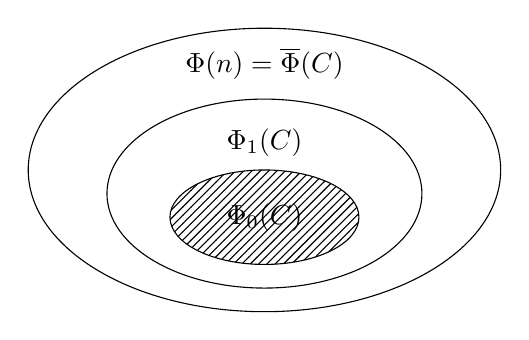
\begin{tikzpicture}[scale=1.0]
        \draw (0, 0) ellipse (3cm and 1.8cm);
        \draw (0, -0.3) ellipse (2cm and 1.2cm);
        \draw[fill opacity=0.4, pattern=north east lines] (0, -0.6) ellipse (1.2cm and 0.6cm);

        \node at (0.0, -0.6) { $\Phi_0(C)$ };
        \node at (0.0, 0.35) { $\Phi_1(C)$ };
        \node at (0, 1.35) { $\Phi(n) = \overline{\Phi}(C)$ };
    \end{tikzpicture}

    \caption{The $n$-implying sets of $\confg$ are increasing in size. If they grow to the set of all ring colorings $\Phi(n)$, the configuration is D-reducible. }
\end{figure}

However, it can occur that $\overline{\Phi}(\confg) \neq \Phi(n)$. This is the case with the ring $R_5$ with a single vertex on the inside, which only supports 3-colorings. To handle (some) of these configurations, a stronger form of D-reducibility was required. This is where we go to C-reducibility.
\section{C-Reducibility}
\label{sec:creduce}

The original proof of the four color theorem used an unavoidable set of C or D reducible configurations. C-reducibility can be thought of as a stronger but more complicated form of D-reducibility. In 2009, John P. Steinberger gave an unavoidable set of D-reducible configurations. With this, C-reducibility is no longer required to prove the four color theorem. However, the concept of C-reducibility is still insightful. Therefore we explain it here.

\subsection{Definitions}

Recall that D-reducibility required that all possible ring colorings $\Phi(n)$ are in the implying set $\overline{\Phi}(C)$. If a configuration is not D-reducible, then there must be ring colorings in $\Phi(n)$ that are not in $\overline{\Phi}(C)$. These colorings can not be converted to coloring of $C$ by flipping Kempe-chains. It is these colorings that we want to avoid with C-reducibility. By replacing $C$ with a reducer $(S,\sigma)$ consisting of a smaller graph $S$ and a ring contraction $\sigma$ we can avoid these colorings. For this to happen, the un-contracted ring colorings of $(S,\sigma)$ denoted by $\Phi(S, \sigma)$ must be in $\overline{\Phi}(C)$.

\begin{figure}[!h]
    \centering
    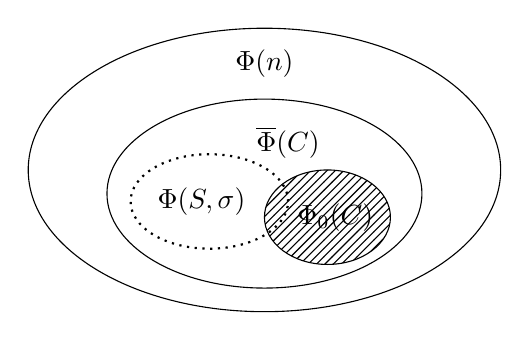
\begin{tikzpicture}[scale=1.0]
        \draw (0, 0) ellipse (3cm and 1.8cm);
        \draw (0, -0.3) ellipse (2cm and 1.2cm);
        \draw[fill opacity=0.4, pattern=north east lines] (0.8, -0.6) ellipse (0.8cm and 0.6cm);
        \draw[dotted, thick] (-0.7, -0.4) ellipse (1.0cm and 0.6cm);

        \node at (0.9, -0.6) { $\Phi_0(C)$ };
        \node at (0.3, 0.35) { $\overline{\Phi}(C)$ };
        \node at (0, 1.35) { $\Phi(n)$ };
        \node at (-0.8, -0.4) { $\Phi(S, \sigma)$ };
    \end{tikzpicture}

    \caption{C-reducibility requires that for some choice of a reducer $(S,\sigma)$, the colorings $\Phi(S, \sigma)$ can be converted to valid ring colorings of $C$ in $\Phi_0(C)$.}
    \label{fig:cred}
\end{figure}

Therefore, C-reducibility can be seen as an extension of D-reducibility with the reducer $(S, \sigma)$ acting as a "filter" of ring colorings. This way we can ignore those ring colorings that are not in $\overline{\Phi}(C)$. As can be seen in Figure \ref{fig:cred}, there are still colorings for the ring that are not in $\overline{\Phi}(C)$. However, we avoid them using the colorings of the reducer $\Phi(S, \sigma)$.

Let us start with the definition of a ring contraction.

\begin{definition}
    A ring contraction $\sigma(v)$ is a map from the vertices of a ring $R$ to the contracted ring $\sigma \circ R$. We require
    
    \begin{itemize}
        \item The contracted ring $\sigma \circ R$ is a valid planar graph.
        \item Neighboring ring vertices $v_i$ and $v_{i+1}$ are not contracted.
    \end{itemize}
\end{definition}

Ring contractions allows the reducer to shrink the number of boundary vertices. This simplifies the coloring problem for the reducer. Without a ring contraction, our reducer would still have the same ring as our configuration $C$, making it equally difficult to work with. Why do we not simply delete vertices from the ring of $C$? The contraction defines a map that allows us to convert boundary colorings of $(S,\sigma)$ to ring colorings of $C$ simply by un-contracting. 

\begin{figure}[!h]
    \centering
    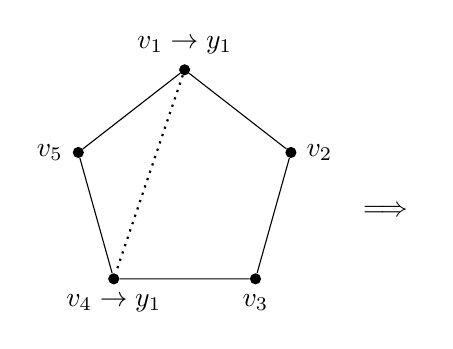
\begin{tikzpicture}[scale=1.5]
        \node[circle, fill, scale=0.015cm, label=above:{$v_1 \rightarrow y_1$}] (l1) at (0, 1) { };
        \node[circle, fill, scale=0.015cm, label=right:{$v_2$}] (l2) at (0.9, 0.30) { };
        \node[circle, fill, scale=0.015cm, label=below:{$v_3$}] (l3) at (0.6, -0.77) {};
        \node[circle, fill, scale=0.015cm, label=below:{$v_4 \rightarrow y_1$}] (l4) at (-0.6, -0.77) {};
        \node[circle, fill, scale=0.015cm, label=left:{$v_5$}] (l5) at (-0.9, 0.30) {};
        \draw (l1) -- (l2) -- (l3) -- (l4) -- (l5) -- (l1);
        \draw[dotted, thick] (l1) -- (l4);
        \node at (1.7, -0.2) { $\implies$ };
    \end{tikzpicture}
    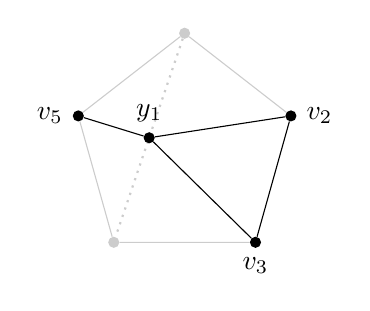
\begin{tikzpicture}[scale=1.5]
        \node[circle, fill, opacity=0.2, scale=0.015cm] (l1) at (0, 1) {};
        \node[circle, fill, opacity=0.2, scale=0.015cm] (l4) at (-0.6, -0.77) {};
        \node[circle, fill, scale=0.015cm, label=above:{$y_1$}] (y1) at (-0.3, 0.115) {};

        \node[circle, fill, scale=0.015cm, label=right:{$v_2$}] (l2) at (0.9, 0.30) { };
        \node[circle, fill, scale=0.015cm, label=below:{$v_3$}] (l3) at (0.6, -0.77) {};
        \node[circle, fill, scale=0.015cm, label=left:{$v_5$}] (l5) at (-0.9, 0.30) {};

        \draw (l5) -- (y1) -- (l2) -- (l3) -- (y1);
        \draw[dotted, thick, opacity=0.2] (l1) -- (l4);
        \draw[opacity=0.2] (l5) -- (l1) -- (l2);
        \draw[opacity=0.2] (l3) -- (l4) -- (l5);
    \end{tikzpicture}
    \caption{A contraction on $R_5$. The two vertices $v_1$ and $v_4$ are mapped to the same vertex $y_1$, and hence get contracted together. }
    \label{fig:contract}
\end{figure}

Figure \ref{fig:contract} shows the contraction process on $R_5$. Intuitively, you should think of a contraction as the merging of pairs of vertices to a single point. However, mathematically, it is easier to work with a mapping function $\sigma$ instead. Suppose we are given a coloring $x(v)$ of a contracted ring $\sigma \circ R$. Then the composition $x \circ \sigma(v)$ is a valid coloring for $R$. This is shown in Figure \ref{fig:contractcolor}

\begin{figure}[!h]
    \centering
    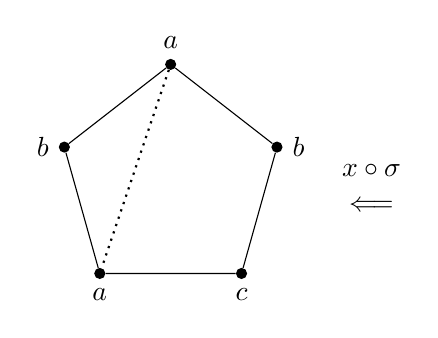
\begin{tikzpicture}[scale=1.5]
        \node[circle, fill, scale=0.015cm, label=above:{$a$}] (l1) at (0, 1) { };
        \node[circle, fill, scale=0.015cm, label=right:{$b$}] (l2) at (0.9, 0.30) { };
        \node[circle, fill, scale=0.015cm, label=below:{$c$}] (l3) at (0.6, -0.77) {};
        \node[circle, fill, scale=0.015cm, label=below:{$a$}] (l4) at (-0.6, -0.77) {};
        \node[circle, fill, scale=0.015cm, label=left:{$b$}] (l5) at (-0.9, 0.30) {};
        \draw (l1) -- (l2) -- (l3) -- (l4) -- (l5) -- (l1);
        \draw[dotted, thick] (l1) -- (l4);
        
        \node at (1.7, 0.1) { $x \circ \sigma$ };
        \node at (1.7, -0.2) { $\Longleftarrow$ };
    \end{tikzpicture}
    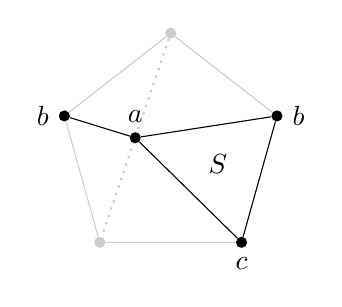
\begin{tikzpicture}[scale=1.5]
        \node[circle, fill, opacity=0.2, scale=0.015cm] (l1) at (0, 1) {};
        \node[circle, fill, opacity=0.2, scale=0.015cm] (l4) at (-0.6, -0.77) {};
        \node[circle, fill, scale=0.015cm, label=above:{$a$}] (y1) at (-0.3, 0.115) {};

        \node[circle, fill, scale=0.015cm, label=right:{$b$}] (l2) at (0.9, 0.30) { };
        \node[circle, fill, scale=0.015cm, label=below:{$c$}] (l3) at (0.6, -0.77) {};
        \node[circle, fill, scale=0.015cm, label=left:{$b$}] (l5) at (-0.9, 0.30) {};

        \draw (l5) -- (y1) -- (l2) -- (l3) -- (y1);
        \draw[dotted, thick, opacity=0.2] (l1) -- (l4);
        \draw[opacity=0.2] (l5) -- (l1) -- (l2);
        \draw[opacity=0.2] (l3) -- (l4) -- (l5);

        \node at (0.4, -0.11) { $S$ };
    \end{tikzpicture}
    \caption{ The coloring $x(v)$ of a contracted ring $\sigma \circ R$ can be converted to a coloring for the original ring $R$ using $x \circ \sigma(v)$. }
    \label{fig:contractcolor}
\end{figure}

By introducing ring contractions, we have already covered the most significant part of a reducer. The last part is the extra graph $S$ that defines the interior of our contracted ring. This extra graph $S$ is similar to the auxiliary graph $A$ that we used during the 1-reducibility proof of $R_5$. The boundary vertices of $S$ must be the same as the contracted ring $\sigma \circ R$. Now we have all the parts needed to define a reducer.

\begin{definition}
    A reducer of a configuration $C$ is a pair $(S, \sigma)$  consisting of a ring contraction $\sigma$ and a graph $S$ on less vertices than $C$ that has a boundary equal to the contracted ring $\sigma \circ R$.
\end{definition}

Of course, every reducer will reduce the size of a configuration $C$. However, for actual reducibility, we can not simply take any reducer. Our reducer $(S, \sigma)$ must satisfy the filtering property mentioned at the beginning of this section. That is, its ring colorings $\Phi(S, \sigma)$ must be contained in $\overline{\Phi}(C)$. Let us define this set.

\begin{definition}
    Let $(S, \sigma)$ be a reducer. The set of un-contracted ring colorings $\Phi(S, \sigma)$ consists of all the colorings $x \circ \sigma$ with $x(v)$ a boundary coloring of $S$.
\end{definition}

Following this definition, C-reducibility is a simple concept.

\begin{definition}
    A configuration $C$ is C-reducible if $\Phi(S,\sigma) \subset \overline{\Phi}(C)$ for some reducer $(S,\sigma)$.
\end{definition}

Now suppose we have a graph $G$ where $C$ is an embedded C-reducible configuration with reducer $(S,\sigma)$. Suppose that two non-neighboring ring vertices of $C$ are connected by an edge in $G$. If we would contract these vertices together, then we would create a loop on the boundary of $S$. We can not color vertices with loops without breaking the rules of a coloring. Therefore, we must take care to avoid such loops.

Since this issue is specific to the way the configuration $C$ is embedded in the graph $G$, we will give a name to the type of embedding that we are after.

\begin{definition}
    A configuration $C$ is $\sigma$-properly embedded in $G$ if two ring vertices of $C$ that are connected by an non-ring edge in $G$ are not contracted by $\sigma(v)$.
\end{definition}

\begin{definition}
    The C-reducible configuration $C$ has a safe reducer  $(S,\sigma)$ if it only occurs $\sigma$-properly embedded in a Birkhoff graph.
\end{definition}

Before we can use C-reducible configurations to reduce counterexamples, we must first prove the existence of a safe reducer. This was a major source of complications in the original proof of the four color theorem by Appel and Haken. This is a strong condition on the structure of a reducer. We will see examples of safe and unsafe reducers in the next section.

\subsection{C-Reducibility of the Birkhoff diamond}
\label{sec:diamond}

Although we have already shown that the Birkhoff diamond is D-reducible, we will use it as a slightly more interesting example of C-reducibility. A reducer for the Birkhoff diamond we have picture below.

\begin{figure}[!h]
    \centering
    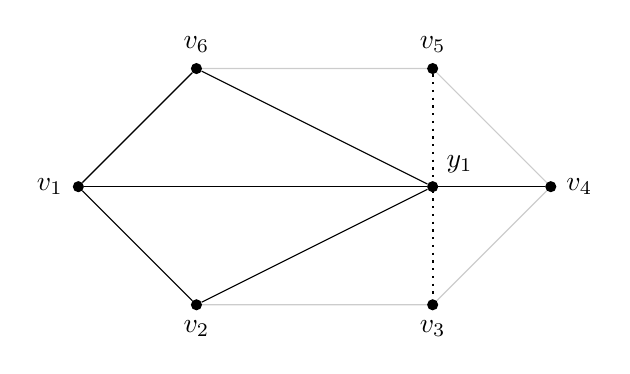
\begin{tikzpicture}[scale=1.5]
        \node[circle, fill, scale=0.015cm, label=left:$v_1$] (l1) at (-2, 0) { };
        \node[circle, fill, scale=0.015cm, label=above:$v_6$] (l2) at (-1, 1) { };
        \node[circle, fill, scale=0.015cm, label=below:$v_2$] (l4) at (-1, -1) {};

        \node[circle, fill, scale=0.015cm,label=right:$v_4$] (r1) at (2, 0) {};
        \node[circle, fill, scale=0.015cm,label=above:$v_5$] (r2) at (1, 1) {};
        \node[circle, fill, scale=0.015cm,label=below:$v_3$] (r4) at (1, -1) {};

        \node[circle, fill, scale=0.015cm,label=above right:$y_1$] (y1) at (1, 0) {};

        \draw[opacity=0.2] (l1) -- (l2) -- (r2) -- (r1) -- (r4) -- (l4) -- (l1);
        \draw[dotted, thick] (r2) -- (r4);
        \draw (l1) -- (l2) -- (y1) -- (l4) -- (l1);
        \draw (l1) -- (y1) -- (r1);
    \end{tikzpicture}
    \caption{A reducer for the Birkhoff diamond (in bold) with a single contraction on $v_4$ and $v_2$, and a single edge added by $S$. }.
    \label{fig:diamondreducer}
\end{figure}

Let us now prove the C-reducibility of the Birkhoff diamond with this reducer. First, we determine the set of colorings that the reducer creates for the original ring $R_6$.

\begin{equation}
    \Phi(S, \sigma) = \left\{ \begin{matrix}
        ababcd, & abcbdc, & abcbcd, \\ abcbac, & abcbad, & \underline{ababac}
    \end{matrix}\right\}
\end{equation}

By looking at Table \
\section{Relating $k$, D and C-Reducibility}
\section{Algorithm}
\label{sec:algorithm}
\section{Conclusions}

\pagebreak
\printbibliography

\end{document}
